\documentclass[../../../../main.tex]{subfiles}
\begin{document}

\begin{flushright}
\footnotesize\textit{【自動文字起こし・要確認】}
\end{flushright}

\begin{center}
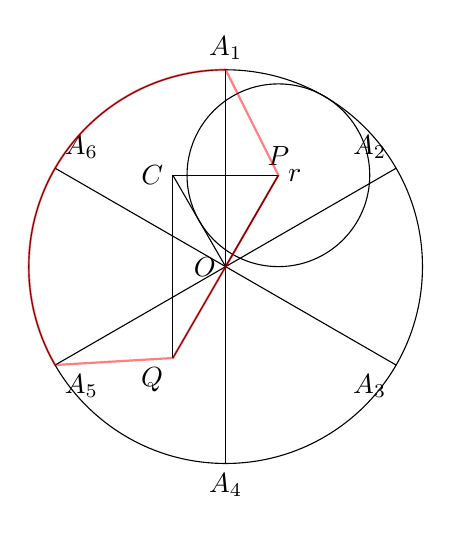
\begin{tikzpicture}[scale=2.5]
    % Coordinates
    \coordinate (O) at (0,0);
    \draw (O) circle (1);
    
    % Radius 1 circle points A1 to A6
    \foreach \i in {1,...,6} {
        \coordinate (A\i) at ({90 - (\i-1)*60}:1);
    }
    
    % Draw radii to A1, A6, A3, A4, A5
    \draw (O) -- (A1) node[above] {$A_1$};
    \draw (O) -- (A6) node[above right] {$A_6$};
    \draw (O) -- (A3) node[below left] {$A_3$};
    \draw (O) -- (A4) node[below] {$A_4$};
    \draw (O) -- (A5) node[below right] {$A_5$};
    \draw (O) -- (A2) node[above left] {$A_2$};

    % Small circle inside angle A1-O-A6
    % Angle is 60 deg, bisector is 60 deg (pi/3) from x-axis, i.e., 60 deg in standard angle (between 90 and 30 deg) -> 60 deg angle relative to origin
    % Radius r = 2\sqrt{3} - 3 \approx 0.4641
    % OP = r / sin(30) = 2r \approx 0.9282 at angle 60 deg
    \coordinate (P) at (60:0.5359); % OP = 1 - r = 1 - 0.4641 = 0.5359
    \draw (P) circle (0.4641);
    \node[above] at (P) {$P$};
    \node[right] at (P) {$r$};

    % Points C, Q
    \coordinate (C) at (120:0.5359);
    \coordinate (Q) at (240:0.5359);
    \coordinate (B) at (0, 0.2);

    \draw (O) -- (P);
    \draw (O) -- (C);
    \draw (P) -- (C);
    \draw (C) -- (Q);
    \draw (P) -- (Q);

    \node[below left] at (Q) {$Q$};
    \node[left] at (C) {$C$};
    \node[left] at (O) {$O$};
    
    % Shaded region indicator
    \draw[thick, red, opacity=0.5] (A1) arc (90:210:1) -- (Q) -- (P) -- cycle;
\end{tikzpicture}
\end{center}

\noindent
\textbf{[解]}

$P$ を中心とする円の半径を $r$ とすると、$OA_1 = OP + PA_1$ より
\[
1 = r + \frac{r}{\sin \frac{\pi}{3}} = \left( \frac{2}{\sqrt{3}} + 1 \right) r = \left( \frac{2}{3}\sqrt{3} + 1 \right) r
\]
\[
\therefore r = -3 + 2\sqrt{3} \quad \cdots \text{①}
\]

題意から、$QC = OP$, $CP = QO$ だから、$\square OPCQ$ は平行四辺形である。

求める面積を $S$ とすると、図形の和・差に分解して考える：

\begin{center}
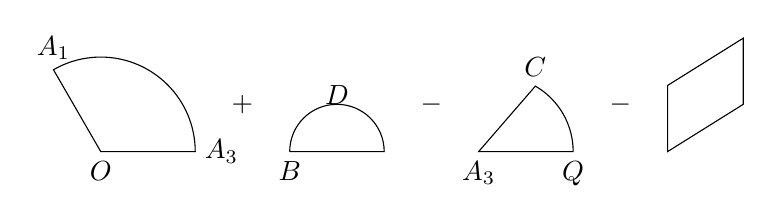
\begin{tikzpicture}[scale=1.2]
    % Diagrams of decomposition
    % Sector OA1A3
    \draw (0,0) node[below]{$O$} -- (1,0) node[right]{$A_3$} arc(0:120:1) node[above]{$A_1$} -- cycle;
    \node at (1.5, 0.5) {$+$};

    % Region D
    \draw (2,0) node[below]{$B$} -- (3,0) arc(0:180:0.5) -- cycle;
    \node at (2.5, 0.6) {$D$};
    \node at (3.5, 0.5) {$-$};

    % Region CQ A3
    \draw (4,0) node[below]{$A_3$} -- (5,0) node[below]{$Q$} arc(0:60:0.8) node[above]{$C$} -- cycle;
    \node at (5.5, 0.5) {$-$};

    % Parallelogram region
    \draw (6,0) -- (6.8, 0.5) -- (6.8, 1.2) -- (6, 0.7) -- cycle;
\end{tikzpicture}
\end{center}

各部分の面積は：
\begin{itemize}
    \item 扇形 $OA_1A_3$: $\frac{1}{2} \cdot \frac{2}{3}\pi = \frac{\pi}{3}$
    \item 半円領域 $D$: $\frac{1}{2}\pi r^2$
    \item 扇形 $Q C A_3$: $\frac{1}{2} \cdot \frac{2}{3}\pi (1-r)^2 = \frac{1}{3}\pi (1-r)^2$
    \item 平行四辺形 $OPCQ$ から扇形を除いた部分:
    \[
    (1-r) \cdot r \cdot \sin \frac{\pi}{3} - \frac{1}{6}\pi r^2 = \frac{\sqrt{3}}{2}(r - r^2) - \frac{1}{6}\pi r^2
    \]
\end{itemize}

だから、代入して
\begin{align*}
S &= \frac{\pi}{3} + \frac{1}{2}\pi r^2 - \frac{1}{3}(1-r)^2\pi - \left\{ \frac{\sqrt{3}}{2}(r-r^2) - \frac{1}{6}\pi r^2 \right\} \\
&= \pi \left\{ \frac{1}{3} + \frac{1}{2}r^2 - \frac{1}{3}(1-r)^2 + \frac{1}{6}r^2 \right\} - \frac{\sqrt{3}}{2}(r-r^2) \\
&= \frac{\pi}{6} \left[ 2r^2 + 4r \right] - \frac{\sqrt{3}}{2} r (1-r)
\end{align*}

ここで、①より $r^2 = (-3+2\sqrt{3})^2 = 21 - 12\sqrt{3}$ だから
\begin{align*}
S &= \frac{\pi}{3} \left\{ (21 - 12\sqrt{3}) + 2(-3 + 2\sqrt{3}) \right\} - \frac{\sqrt{3}}{2} \left\{ (-3 + 2\sqrt{3}) - (21 - 12\sqrt{3}) \right\} \\
&= \frac{\pi}{3} \left[ 15 - 8\sqrt{3} \right] - \frac{\sqrt{3}}{2} \left( -24 + 14\sqrt{3} \right) \\
&= (15 - 8\sqrt{3})\frac{\pi}{3} - 21 + 12\sqrt{3} \\
&= (5\pi - 21) + \left( 12 - \frac{8}{3}\pi \right)\sqrt{3}
\end{align*}

\newpage

\end{document}
